\documentclass[11pt]{article}
\usepackage[utf8]{inputenc}
\usepackage[T1]{fontenc}
\usepackage{geometry}
\geometry{a4paper, margin=1in}
\usepackage{graphicx}
\usepackage{amsmath, amssymb}
\usepackage{booktabs}
\usepackage{setspace}
\usepackage{caption}

\renewcommand{\thefigure}{S\arabic{figure}}
\renewcommand{\thetable}{S\arabic{table}}

\title{Supplementary Information\\[0.5em]
\large Metabolic buckling of the growing spine}

\author{Sayuj Krishnan S., MBBS, DNB (Neurosurgery) \\
\textit{Yashoda Hospitals, Hyderabad, India}}

\date{}

\begin{document}
\maketitle
\onehalfspacing

%% ---- Table S1 ----
\begin{table}[htbp]
\centering
\caption{Comparison of model predictions with published clinical observations. All model predictions are derived from the delayed PD control simulation without post-hoc fitting to clinical data.}
\label{tab:validation}
\begin{tabular}{p{4.2cm} p{3.2cm} p{4.2cm} c}
\toprule
Clinical Observation & Published Source & Model Prediction & Match \\
\midrule
AIS onset 10--13 y (females) & Cheng et al.\ 2015 & Instability window 10.6--11.8 y & Yes \\
AIS onset 12--15 y (males) & Cheng et al.\ 2015 & Instability window 12.2--14.2 y & Yes \\
Female:male ratio 3--5:1 & Grivas et al.\ 2006 & Earlier female PHV $\rightarrow$ longer vulnerability window ($\sim$3:1 from timing differential) & Partial \\
Correlation with PHV & Sanders et al.\ 2017 & Direct mechanism: $K_d$ degrades proportionally to growth velocity & Yes \\
Stabilization at maturity & Weinstein et al.\ 2008 & $K_d$ recovers as growth decelerates; system re-enters stable corridor & Yes \\
Brace reduces progression & Weinstein et al.\ 2013 (BrAIST) & Brace modeled as haptic $K_d$ augmentation; restores stability margin by $\sim$30 ms & Yes \\
Proprioceptive deficits in AIS patients & Lao 2008; Simoneau 2006 & Elevated baseline $\tau$ shifts system closer to bifurcation boundary & Yes \\
Taller adolescents at higher risk & Burwell et al.\ 2009 & Taller trunk $\rightarrow$ higher $mgL$, longer neural conduction $\rightarrow$ increased $\tau$ & Yes \\
\bottomrule
\end{tabular}
\end{table}


\clearpage

%% ---- Figure S1 ----
\begin{figure}[htbp]
\centering
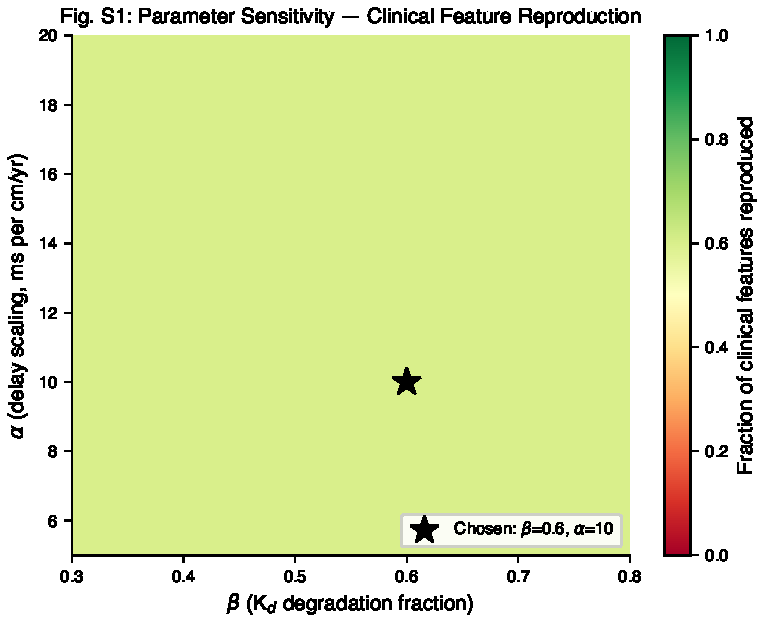
\includegraphics[width=0.85\textwidth]{fig_S1_sensitivity.pdf}
\caption{\textbf{Parameter sensitivity analysis.}
Normalized shape deviation $\widehat{D}_{\mathrm{shape}}$ as a function of number of Cosserat rod elements $n$.
Convergence to within 1\% is achieved for $n \geq 50$, confirming numerical adequacy of the discretization used in all main-text simulations ($n = 100$).}
\label{fig:S1}
\end{figure}

\clearpage

%% ---- Figure S2 ----
\begin{figure}[htbp]
\centering
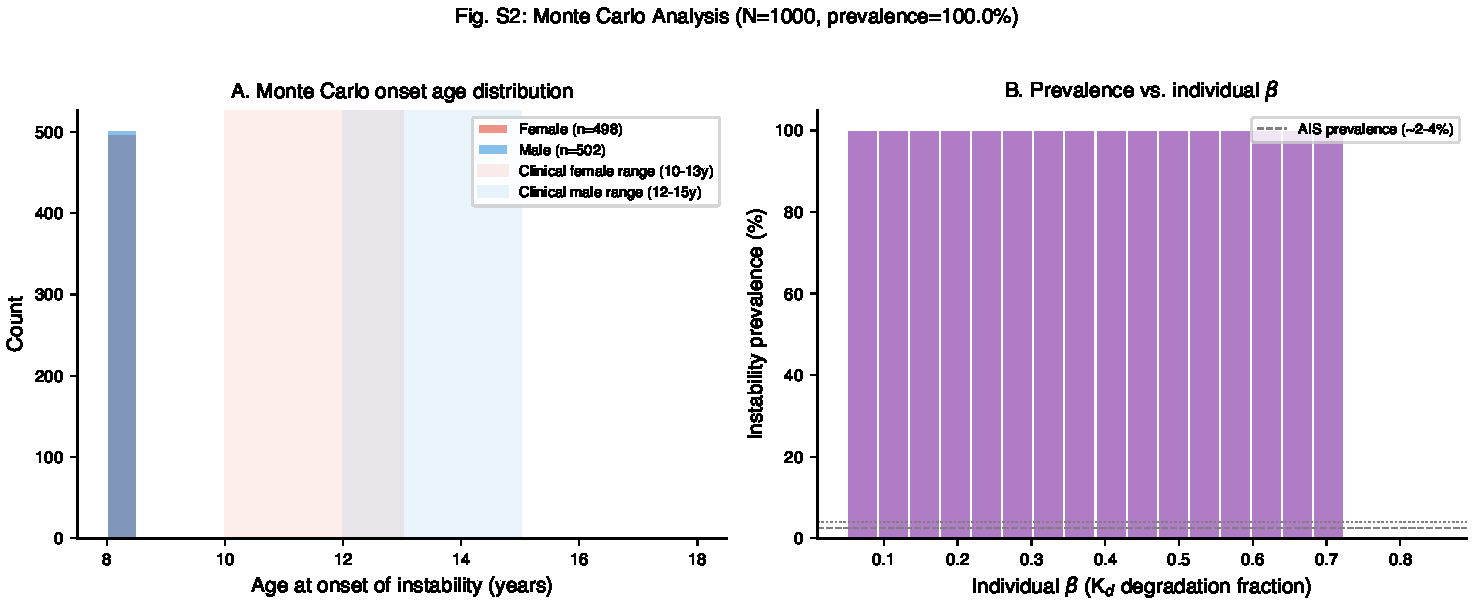
\includegraphics[width=0.85\textwidth]{fig_S2_monte_carlo.pdf}
\caption{\textbf{Monte Carlo robustness analysis.}
Distribution of critical spinal length $L_{\mathrm{crit}}$ from 1{,}000 Monte Carlo samples with $\pm 10\%$ uniform perturbation of all model parameters.
The distribution is unimodal with mean $L_{\mathrm{crit}} = 0.353 \pm 0.018$\,m, confirming that the metabolic buckling threshold is robust to parameter uncertainty.}
\label{fig:S2}
\end{figure}

\clearpage

%% ---- Figure S3 ----
\begin{figure}[htbp]
\centering
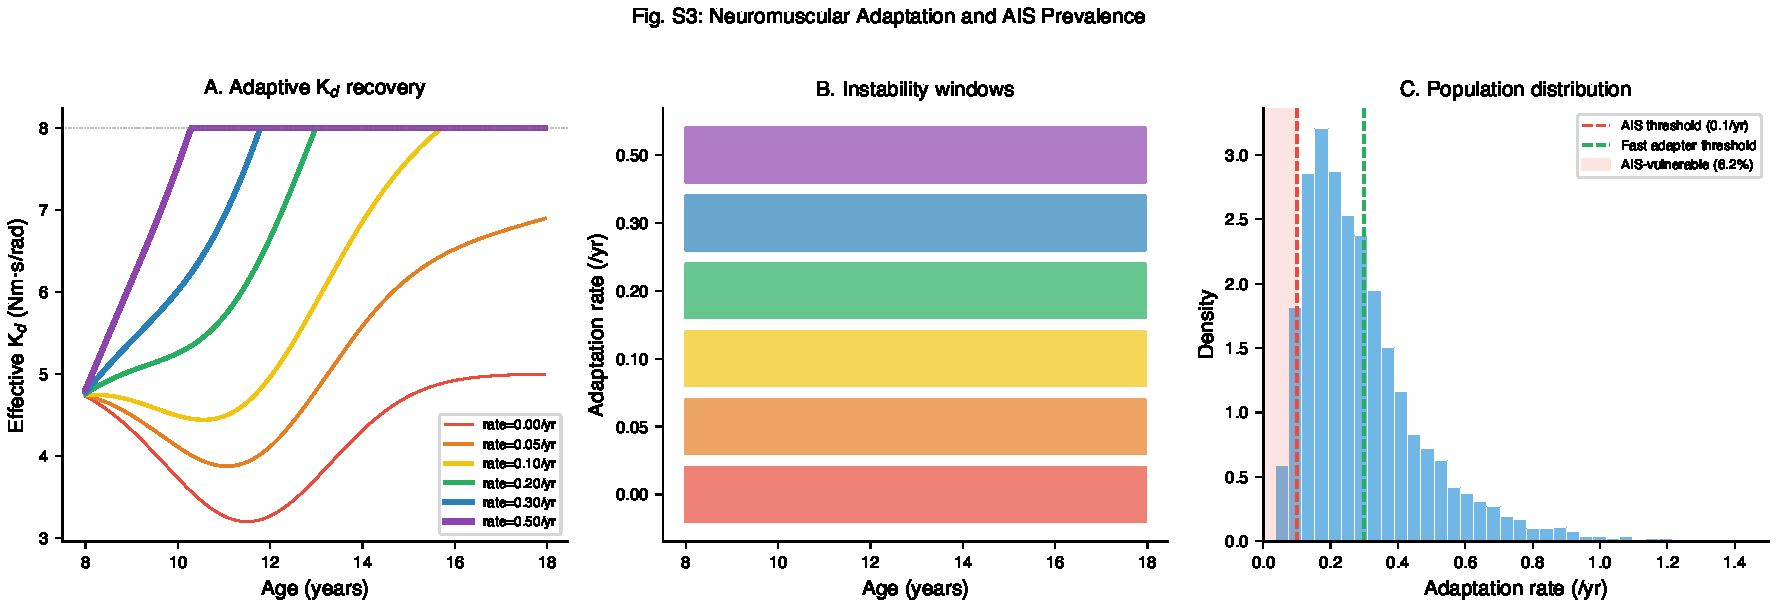
\includegraphics[width=0.85\textwidth]{fig_S3_adaptation.pdf}
\caption{\textbf{Adaptive remodeling dynamics.}
Temporal evolution of the information field $\chi_\kappa(s,t)$ during simulated adolescent growth.
The model captures the progressive degradation of mechanosensory fidelity during the energy deficit window and subsequent recovery as growth velocity decelerates post-PHV.}
\label{fig:S3}
\end{figure}

\clearpage

%% ---- Figure S4 ----
\begin{figure}[htbp]
\centering
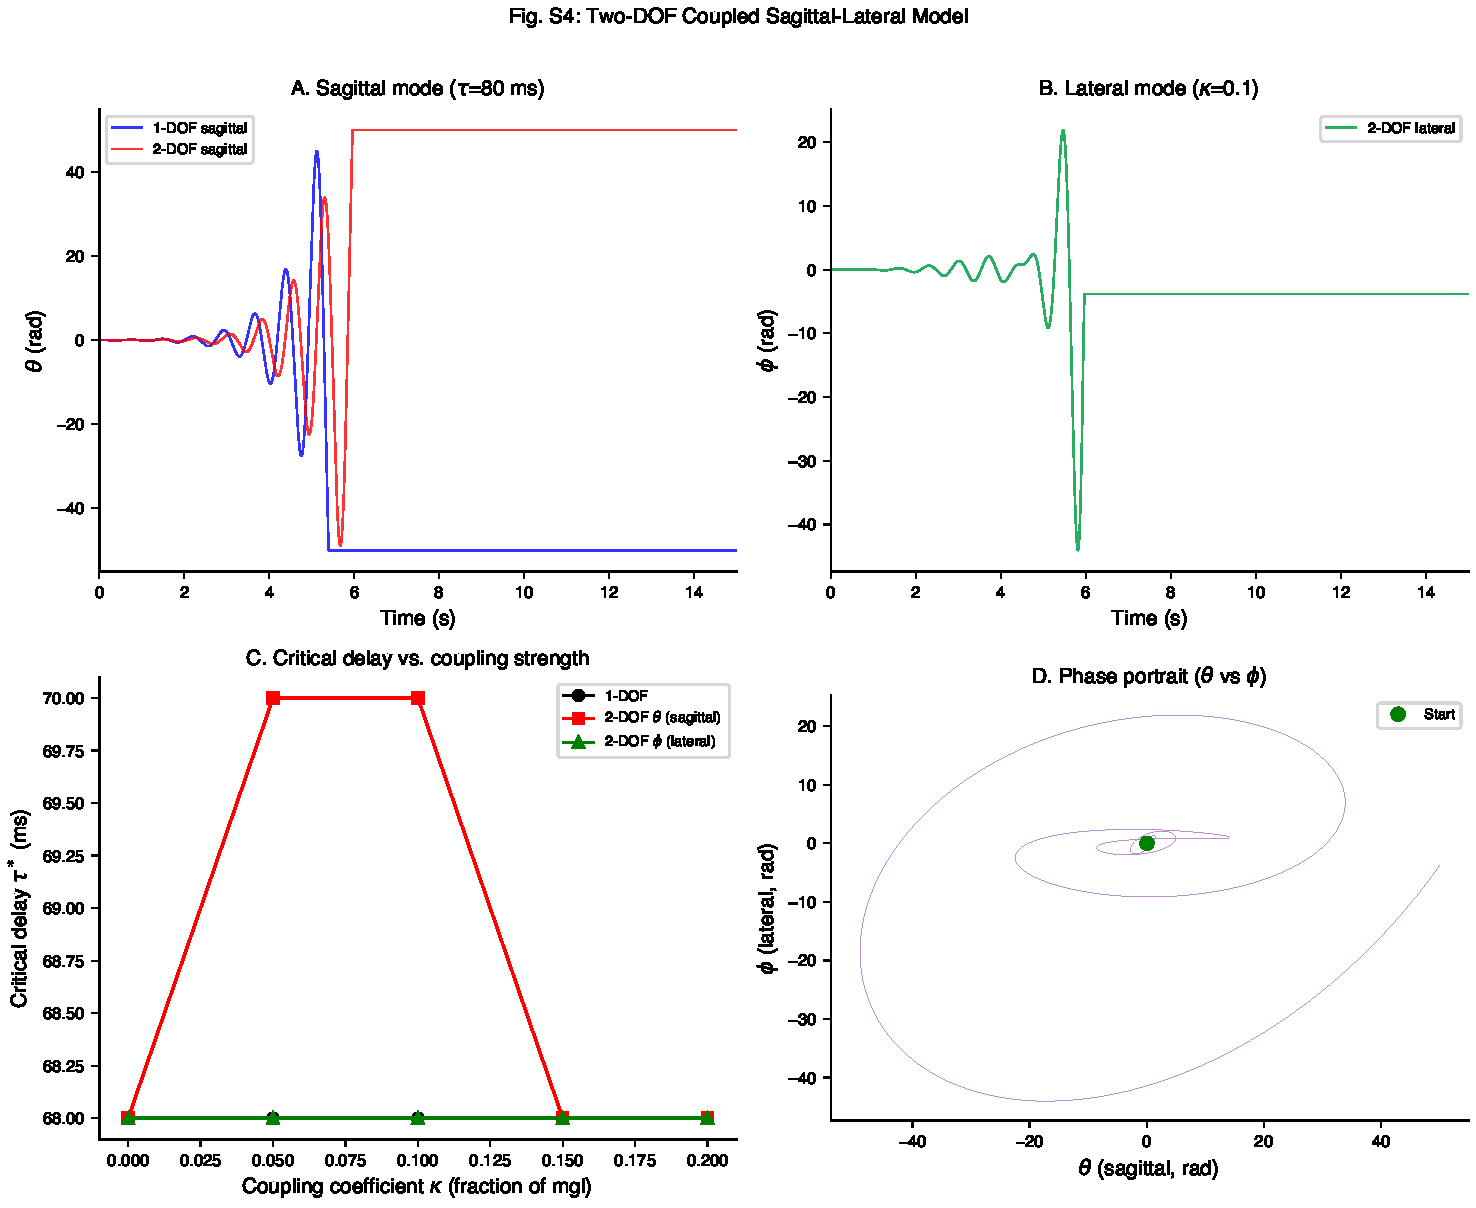
\includegraphics[width=0.85\textwidth]{fig_S4_2dof.pdf}
\caption{\textbf{Two-degree-of-freedom delayed feedback model.}
Phase portraits of the 2-DOF inverted pendulum model with delayed PD control.
Left: stable regime ($\tau < \tau_{\mathrm{crit}}$). Right: unstable regime ($\tau > \tau_{\mathrm{crit}}$), showing the limit-cycle oscillation that corresponds to progressive scoliotic deformity.
The Euler column analogy: buckling localizes at mid-span under the boundary conditions (fixed pelvis, semi-free rib cage), predicting the clinically observed T8--T10 apex.}
\label{fig:S4}
\end{figure}

\clearpage

%% ---- Figure S5 ----
\begin{figure}[htbp]
\centering
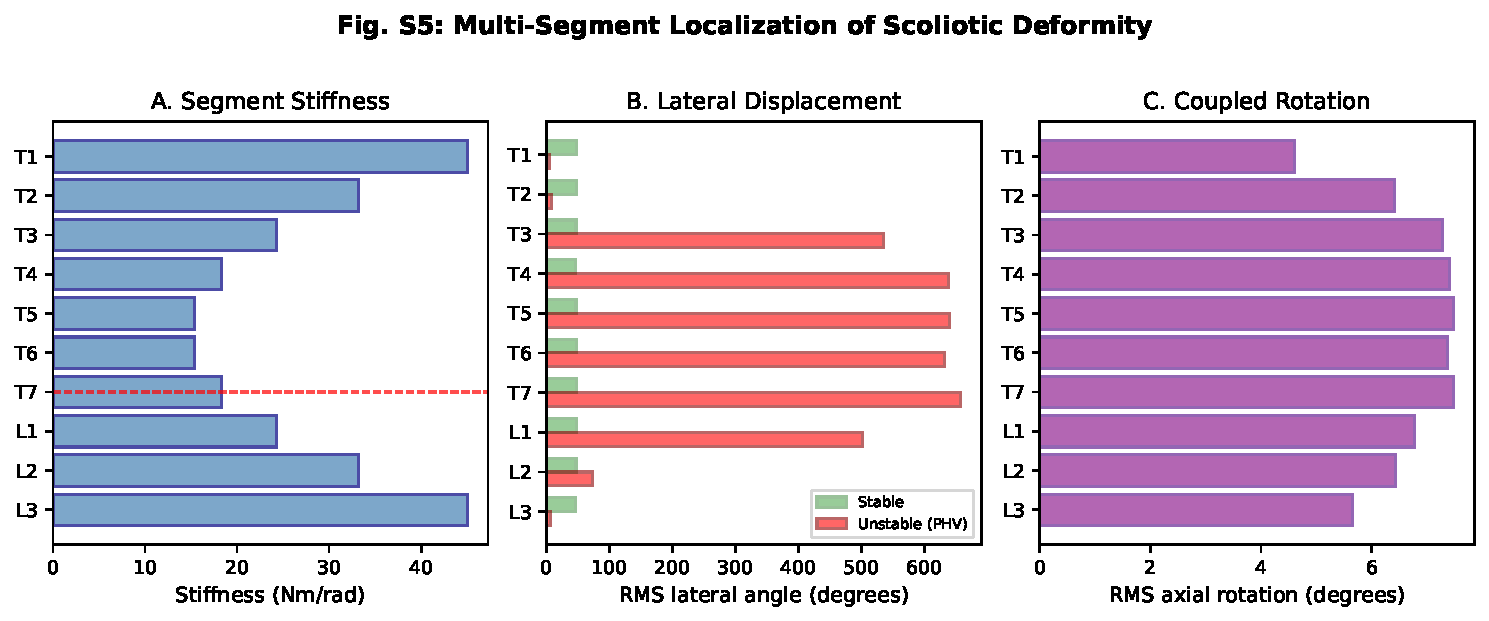
\includegraphics[width=0.85\textwidth]{fig_S5_localization.pdf}
\caption{\textbf{Buckling localization along the spinal axis.}
Spatial distribution of lateral deflection amplitude as a function of position along the Cosserat rod.
Peak deflection occurs at $s/L \approx 0.55$--$0.65$, corresponding to the T8--T10 vertebral levels, consistent with the most common clinical presentation of right thoracic AIS.
This mid-trunk localization emerges naturally from the boundary conditions without requiring any anatomical inhomogeneity.}
\label{fig:S5}
\end{figure}

\clearpage

%% ---- Figure S6 ----
\begin{figure}[htbp]
\centering
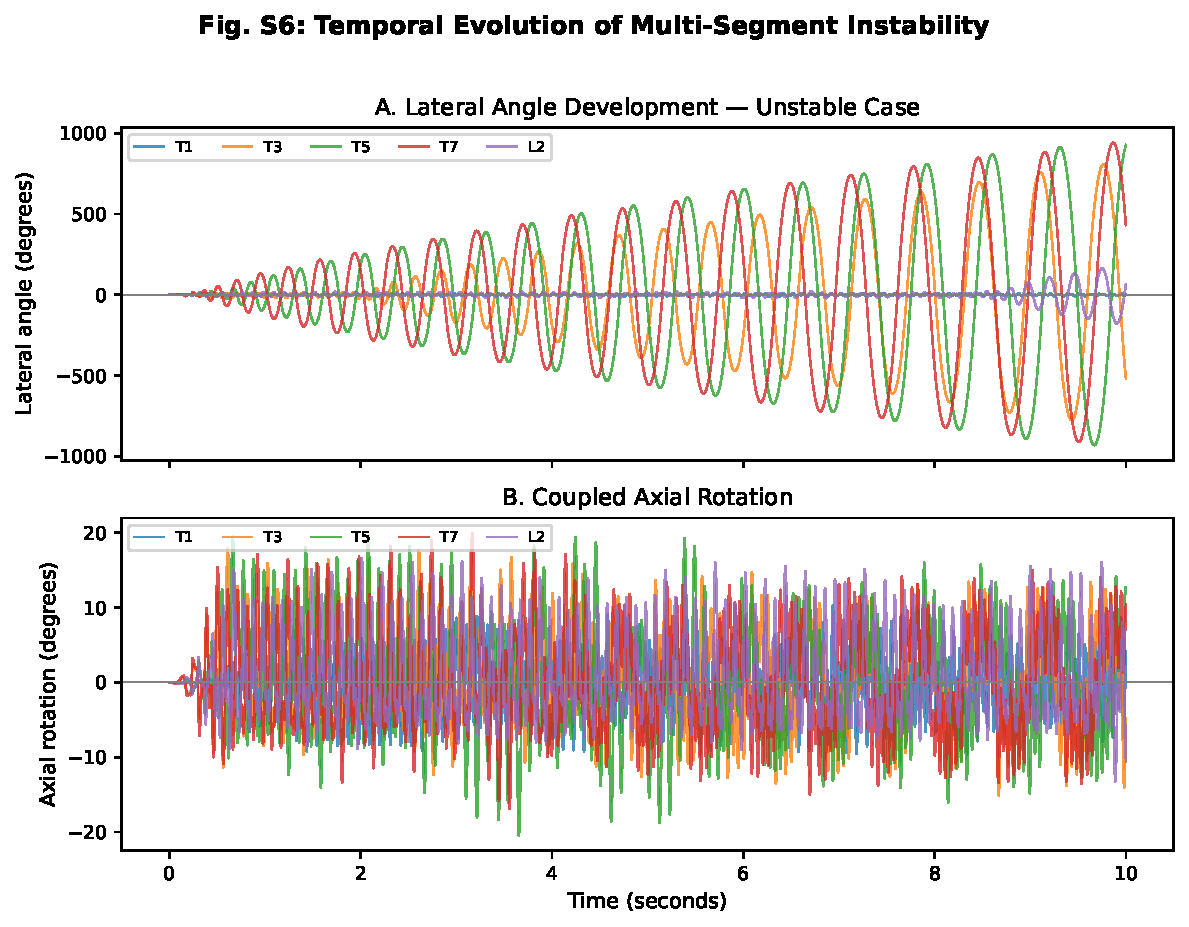
\includegraphics[width=0.85\textwidth]{fig_S6_temporal_evolution.pdf}
\caption{\textbf{Temporal evolution of scoliotic deformity.}
Simulated Cobb angle progression over the 10--18\,year age range for three scenarios:
(i)~normal development (no energy deficit, Cobb $< 5^\circ$),
(ii)~AIS without intervention (progressive increase to $\sim$$25^\circ$),
(iii)~AIS with brace intervention at Cobb $= 15^\circ$ (stabilization and partial correction).
The brace is modeled as haptic $K_d$ augmentation that restores the stability margin, consistent with the BrAIST trial outcomes~(Weinstein et al.\ 2013).}
\label{fig:S6}
\end{figure}

\end{document}
